% Options for packages loaded elsewhere
\PassOptionsToPackage{unicode}{hyperref}
\PassOptionsToPackage{hyphens}{url}
\PassOptionsToPackage{dvipsnames,svgnames,x11names}{xcolor}
%
\documentclass[
  letterpaper,
  DIV=11,
  numbers=noendperiod]{scrartcl}

\usepackage{amsmath,amssymb}
\usepackage{iftex}
\ifPDFTeX
  \usepackage[T1]{fontenc}
  \usepackage[utf8]{inputenc}
  \usepackage{textcomp} % provide euro and other symbols
\else % if luatex or xetex
  \usepackage{unicode-math}
  \defaultfontfeatures{Scale=MatchLowercase}
  \defaultfontfeatures[\rmfamily]{Ligatures=TeX,Scale=1}
\fi
\usepackage{lmodern}
\ifPDFTeX\else  
    % xetex/luatex font selection
\fi
% Use upquote if available, for straight quotes in verbatim environments
\IfFileExists{upquote.sty}{\usepackage{upquote}}{}
\IfFileExists{microtype.sty}{% use microtype if available
  \usepackage[]{microtype}
  \UseMicrotypeSet[protrusion]{basicmath} % disable protrusion for tt fonts
}{}
\makeatletter
\@ifundefined{KOMAClassName}{% if non-KOMA class
  \IfFileExists{parskip.sty}{%
    \usepackage{parskip}
  }{% else
    \setlength{\parindent}{0pt}
    \setlength{\parskip}{6pt plus 2pt minus 1pt}}
}{% if KOMA class
  \KOMAoptions{parskip=half}}
\makeatother
\usepackage{xcolor}
\setlength{\emergencystretch}{3em} % prevent overfull lines
\setcounter{secnumdepth}{-\maxdimen} % remove section numbering
% Make \paragraph and \subparagraph free-standing
\ifx\paragraph\undefined\else
  \let\oldparagraph\paragraph
  \renewcommand{\paragraph}[1]{\oldparagraph{#1}\mbox{}}
\fi
\ifx\subparagraph\undefined\else
  \let\oldsubparagraph\subparagraph
  \renewcommand{\subparagraph}[1]{\oldsubparagraph{#1}\mbox{}}
\fi


\providecommand{\tightlist}{%
  \setlength{\itemsep}{0pt}\setlength{\parskip}{0pt}}\usepackage{longtable,booktabs,array}
\usepackage{calc} % for calculating minipage widths
% Correct order of tables after \paragraph or \subparagraph
\usepackage{etoolbox}
\makeatletter
\patchcmd\longtable{\par}{\if@noskipsec\mbox{}\fi\par}{}{}
\makeatother
% Allow footnotes in longtable head/foot
\IfFileExists{footnotehyper.sty}{\usepackage{footnotehyper}}{\usepackage{footnote}}
\makesavenoteenv{longtable}
\usepackage{graphicx}
\makeatletter
\def\maxwidth{\ifdim\Gin@nat@width>\linewidth\linewidth\else\Gin@nat@width\fi}
\def\maxheight{\ifdim\Gin@nat@height>\textheight\textheight\else\Gin@nat@height\fi}
\makeatother
% Scale images if necessary, so that they will not overflow the page
% margins by default, and it is still possible to overwrite the defaults
% using explicit options in \includegraphics[width, height, ...]{}
\setkeys{Gin}{width=\maxwidth,height=\maxheight,keepaspectratio}
% Set default figure placement to htbp
\makeatletter
\def\fps@figure{htbp}
\makeatother
% definitions for citeproc citations
\NewDocumentCommand\citeproctext{}{}
\NewDocumentCommand\citeproc{mm}{%
  \begingroup\def\citeproctext{#2}\cite{#1}\endgroup}
\makeatletter
 % allow citations to break across lines
 \let\@cite@ofmt\@firstofone
 % avoid brackets around text for \cite:
 \def\@biblabel#1{}
 \def\@cite#1#2{{#1\if@tempswa , #2\fi}}
\makeatother
\newlength{\cslhangindent}
\setlength{\cslhangindent}{1.5em}
\newlength{\csllabelwidth}
\setlength{\csllabelwidth}{3em}
\newenvironment{CSLReferences}[2] % #1 hanging-indent, #2 entry-spacing
 {\begin{list}{}{%
  \setlength{\itemindent}{0pt}
  \setlength{\leftmargin}{0pt}
  \setlength{\parsep}{0pt}
  % turn on hanging indent if param 1 is 1
  \ifodd #1
   \setlength{\leftmargin}{\cslhangindent}
   \setlength{\itemindent}{-1\cslhangindent}
  \fi
  % set entry spacing
  \setlength{\itemsep}{#2\baselineskip}}}
 {\end{list}}
\usepackage{calc}
\newcommand{\CSLBlock}[1]{\hfill\break\parbox[t]{\linewidth}{\strut\ignorespaces#1\strut}}
\newcommand{\CSLLeftMargin}[1]{\parbox[t]{\csllabelwidth}{\strut#1\strut}}
\newcommand{\CSLRightInline}[1]{\parbox[t]{\linewidth - \csllabelwidth}{\strut#1\strut}}
\newcommand{\CSLIndent}[1]{\hspace{\cslhangindent}#1}

\KOMAoption{captions}{tableheading}
\makeatletter
\@ifpackageloaded{caption}{}{\usepackage{caption}}
\AtBeginDocument{%
\ifdefined\contentsname
  \renewcommand*\contentsname{Table of contents}
\else
  \newcommand\contentsname{Table of contents}
\fi
\ifdefined\listfigurename
  \renewcommand*\listfigurename{List of Figures}
\else
  \newcommand\listfigurename{List of Figures}
\fi
\ifdefined\listtablename
  \renewcommand*\listtablename{List of Tables}
\else
  \newcommand\listtablename{List of Tables}
\fi
\ifdefined\figurename
  \renewcommand*\figurename{Figure}
\else
  \newcommand\figurename{Figure}
\fi
\ifdefined\tablename
  \renewcommand*\tablename{Table}
\else
  \newcommand\tablename{Table}
\fi
}
\@ifpackageloaded{float}{}{\usepackage{float}}
\floatstyle{ruled}
\@ifundefined{c@chapter}{\newfloat{codelisting}{h}{lop}}{\newfloat{codelisting}{h}{lop}[chapter]}
\floatname{codelisting}{Listing}
\newcommand*\listoflistings{\listof{codelisting}{List of Listings}}
\usepackage{amsthm}
\theoremstyle{plain}
\newtheorem{proposition}{Proposition}[section]
\theoremstyle{remark}
\AtBeginDocument{\renewcommand*{\proofname}{Proof}}
\newtheorem*{remark}{Remark}
\newtheorem*{solution}{Solution}
\newtheorem{refremark}{Remark}[section]
\newtheorem{refsolution}{Solution}[section]
\makeatother
\makeatletter
\makeatother
\makeatletter
\@ifpackageloaded{caption}{}{\usepackage{caption}}
\@ifpackageloaded{subcaption}{}{\usepackage{subcaption}}
\makeatother
\ifLuaTeX
  \usepackage{selnolig}  % disable illegal ligatures
\fi
\usepackage{bookmark}

\IfFileExists{xurl.sty}{\usepackage{xurl}}{} % add URL line breaks if available
\urlstyle{same} % disable monospaced font for URLs
\hypersetup{
  pdftitle={Spurious Sentience},
  pdfauthor={Patrick Altmeyer},
  colorlinks=true,
  linkcolor={blue},
  filecolor={Maroon},
  citecolor={Blue},
  urlcolor={Blue},
  pdfcreator={LaTeX via pandoc}}

\title{Spurious Sentience}
\usepackage{etoolbox}
\makeatletter
\providecommand{\subtitle}[1]{% add subtitle to \maketitle
  \apptocmd{\@title}{\par {\large #1 \par}}{}{}
}
\makeatother
\subtitle{On the Unsurprising Finding of Patterns in Latent Spaces}
\author{Patrick Altmeyer}
\date{2024-01-10}

\begin{document}
\maketitle

\emph{For the slides see \href{slides.qmd}{here}.}

We humans are prone to seek patterns everywhere. Meaningful patterns
have often proven to help us make sense of our past, navigate our
presence and predict the future. Our society is so invested in finding
patterns that today it seems we are more willing than ever to outsource
this task to an Artificial Intelligence (AI): an omniscient oracle that
leads us down the right path. Unfortunately, history has shown time and
again that patterns are double-edged swords: if we attribute the wrong
meaning to them, they may lead us nowhere at all, or worse, they may
lead us down the dark roads.

In statistics, misleading patterns are referred to as \textbf{spurious
relationships}: purely associational relationships between two or more
variables that are not causally related to each other at all. The world
is full of these and as good as we as species may be at recognizing
patterns, we typically have a much harder time discerning spurious
relationships from causal ones. Despite new and increased momentum in
scientific fields concerned with causal inference and discovery, I am
also willing to go out on a limb and claim that we are not about to
finally reach the top of Judea Pearl's Causal Ladder through the means
of Causal AI.

I agree with the premise that in a world full of spurious relationships,
causal reasoning is our only remedy. But I am very skeptical of claims
that AI will magically provide that remedy. This leads me to the title
and topic of this post: \textbf{spurious sentience}---patterns exhibited
by artificial intelligence that may hint at sentience but are just
reflections of the data used to train them. The article is written in
response to a recent paper that extracts a `world model' from Llama
2---a popular open-source large language model (LLM)---using mechanistic
interpretability (Gurnee and Tegmark 2023). In light of these findings,
one of the authors, Max Tegmark, was quick to claim on
\href{https://x.com/tegmark/status/1709572469978231063?s=20}{social
media} that ``No, LLM's aren't mere stochastic parrots {[}\ldots{]}''.

Since this is an opinionated post, I feel that I should start with a few
disclaimers:

\begin{enumerate}
\def\labelenumi{\arabic{enumi}.}
\tightlist
\item
  I take no issue with the methodological ideas that form the foundation
  of the article in question: on the contrary, I think that mechanistic
  interpretability is an interesting and important toolkit that can help
  us better understand the intrinsics and behavior of opaque artificial
  intelligence.
\item
  The visualizations are intriguing, the code is open-sourced and the
  findings are interesting.
\item
  I am surprised that people are surprised by the findings: if we agree
  that LLMs exhibit strong capabilities that can only be connected to
  the patterns observed in the data they were trained with, then where
  exactly should we expect this information to be stored if not in the
  parameters of the model?\footnote{I would be very
    surprised---concerned even---if our search for patterns in latent
    spaces of capable LLMs revealed nothing at all.}
\item
  I therefore do take issue with the way that these findings are being
  overblown by people with clout. Perhaps the parrot metaphor should not
  be taken too literally either, but if anything the paper's findings
  seem to support the notion that LLMs are remarkably capable of
  memorizing and regurgitating explicit and implicit knowledge contained
  in text.
\end{enumerate}

\subsection{Patterns in Latent Spaces and How to Find
Them}\label{patterns-in-latent-spaces-and-how-to-find-them}

To support my claim that observing patterns in latent spaces should not
generally surprise us, we will now go through a couple of simple
examples. To illustrate further that this phenomenon is neither
surprising nor unique to the field of computer science, I will draw on
my background in economics and finance in this section. We will start
with very simple examples to demonstrate that even small and simple
models can learn meaningful representations of the data. The final
example in \textbf{?@sec-ex-llm} is a bit more involved and closer in
spirit to the experiments conducted by Gurnee and Tegmark (2023). As we
go along, we will try to discuss both the benefits and potential
pitfalls of finding patterns in latent spaces.

\subsubsection{Example: Principal Component
Analysis}\label{example-principal-component-analysis}

In response to the claims made by Tegmark, numerous commentators on
social media have pointed out that even the simplest of models can
exhibit structure in their latent spaces. One of the most popular and
illustrative examples I remember from my time at the Bank of England is
yield curve decomposition through PCA. The yield curve is a popular tool
for investors and economists to gauge the health of the economy. It
plots the yields of bonds against their maturities. The slope of the
yield curve is often used as a predictor of future economic activity: a
steep yield curve is associated with a growing economy, while a flat or
inverted yield curve is associated with a contracting economy.

To understand this better, let us go on a quick detour into economics
and look at actual yield curves observed in the US during the Global
Financial Crisis (GFC). Figure~\ref{fig-gfc-1} shows the yield curve of
US Treasury bonds on 27 February 2007, which according to
\href{https://money.cnn.com/2007/02/27/markets/markets_0630/index.htm?cnn=yes}{CNN}
was a ``brutal day on Wall Street''.\footnote{The
  \href{https://home.treasury.gov/resource-center/data-chart-center/interest-rates/TextView?type=daily_treasury_yield_curve&field_tdr_date_value_month=202310}{data}
  is taken from the US Department of the Treasury.} This followed
\href{https://money.cnn.com/2007/02/26/news/economy/greenspan/index.htm?postversion=2007022609}{reports}
on the previous day of former Federal Reserve Chairman Alan Greenspan's
warning that the US economy was at risk of a recession. The yield curve
was inverted with a sharp negative spread between the 10-year and
3-month yields, indicative of the market's expectation of a recession.

Figure~\ref{fig-gfc-2} shows the corresponding yield curve during the
aftermath of the GFC on 20 April 2009. On that day the influential Time
Magazine
\href{https://content.time.com/time/business/article/0,8599,1890560,00.html}{reported}
that the ``Banking Crisis is Over''. The yield curve was steeply sloped
with a positive spread between the 10-year and 3-month yields,
indicative of the market's expectation of a recovery. The overall level
of the yield curve was still very low though, indicative of the fact
that US economy had not fully recovered at that point.

\begin{figure}

\begin{minipage}{\linewidth}

\centering{

\includegraphics{index_files/mediabag/index_files/figure-pdf/fig-gfc-output-1.pdf}

}

\subcaption{\label{fig-gfc-1}Onset of GFC: 27 February 2007.}

\end{minipage}%
\newline
\begin{minipage}{\linewidth}

\centering{

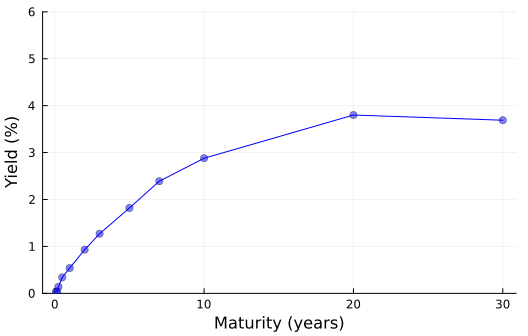
\includegraphics{index_files/mediabag/index_files/figure-pdf/fig-gfc-output-2.pdf}

}

\subcaption{\label{fig-gfc-2}Aftermath of GFC: 20 April 2009.}

\end{minipage}%

\caption{\label{fig-gfc}Yield curve of US Treasury bonds.}

\end{figure}%

Of course, US Treasuries are not the only bonds that are traded in the
market. To get a more complete picture of the economy, analysts might
therefore be interested in looking at the yield curves of other bonds as
well. In particular, we might be interested in predicting economic
growth based on the yield curves of many different bonds. The problem
with that idea is that it is cursed by high dimensionality: we would end
up modelling a single variable of interest (economic growth) with a
large number of predictors (the yields of many different bonds). To deal
with the curse of high dimensionality it can be useful to decompose the
yield curves into sets of principal components.

To compute the principal components we can decompose the matrix of
yields \(\mathbf{Y}\) into a product of its singular vectors and values:
\(\mathbf{Y}=\mathbf{U}\Sigma\mathbf{V}^{\prime}\). I will not go into
the details here, because Professor Gilbert Strang has already done a
much better job than I ever could in his
\href{https://www.youtube.com/watch?v=mBcLRGuAFUk}{Linear Algebra
lectures}. To put this into the broader context of the article, however,
let us simply refer to \(\mathbf{U}\), \(\Sigma\) and
\(\mathbf{V}^{\prime}\) as latent embeddings of the yield curve (they
are latent because they are not directly observable).

The top panel in Figure~\ref{fig-pca} shows the first two principal
components of the yield curves of US Treasury bonds over time. Vertical
stalks indicate the key dates during the onset and aftermath of the
crisis, which we discussed above. For both components, we can observe
some marked shifts between the two dates - but can we attribute any
meaning to these shifts? It turns out we can: for comparison, the bottom
panel in Figure~\ref{fig-pca} shows the average level and spread of the
yield curves over time. The first principal component is strongly
correlated with the level of the yield curve, while the second principal
component is strongly correlated with the spread of the yield curve. To
put it in AI-lingo:

\begin{quote}
The estimated latent embeddings of the yield curve are characterized by
patterns observed in the data.
\end{quote}

\begin{figure}

\centering{

\includegraphics{results/figures/pca.png}

}

\caption{\label{fig-pca}Comparison of latent embeddings and observed
data of the US Treasury yield curve.}

\end{figure}%

Not convinced? Let us use
\(\mathbf{Y}=\mathbf{U}\Sigma\mathbf{V}^{\prime}\) in true autoencoder
fashion to reconstruct yield curves from principal components. Let
\(z_1\) denote the first principal component and consider the following:
we keep all other \(M-1\) principal components fixed at zero where \(M\)
denotes the total number of maturities; next we traverse the latent
space by varying the value of \(z_1\) over a fixed grid of length \(K\)
each time storing the full vector \(\mathbf{z}\); finally, we vertically
concatenate the vectors and end up with a matrix \(\mathbf{Z}\) of
dimension \((K \times M)\). To reconstruct yields, we simply multiply
\(Z\) by the singular values and right singular vectors:
\(\mathbf{Y}=\mathbf{Z}\Sigma\mathbf{V}^{\prime}\).

\textbf{?@fig-pca-anim} shows the result of this exercise in the left
panel. As we can see, our generated yield curves shift vertically as we
traverse the latent space. The right panel of \textbf{?@fig-pca-anim}
shows the result of a similar exercise, but this time we keep the first
principal component fixed at zero and vary the second principal
component. This time the slope of our generated yield curves shifts as
we traverse the latent space.

\subsubsection{Example: Deep Learning}\label{example-deep-learning}

So far we have considered simple matrix decomposition. You might argue
that principal components are not really latent embeddings in the
traditional sense of deep learning. To address this, let us now consider
a simple deep-learning example. Our goal will be to not only predict
economic growth from the yield curve but also extract meaningful
features at the same time. In particular, we will use a neural network
architecture that allows us to recover a compressed latent
representation of the yield curve.

\paragraph{Data}\label{data}

To estimate economic growth we will rely on a quarterly
\href{https://fred.stlouisfed.org/series/GDPC1}{series} of the real
gross domestic product (GDP) provided by the Federal Reserve Bank of
St.~Louis. The data arrives in terms of levels of real GDP. In order to
estimate growth, we will transform the data into log differences. Since
our yield curve data is daily, we will need to aggregate it to the
quarterly frequency. To do this, we will simply take the average of the
daily yields for each maturity. We will also standardize yields since
deep learning models tend to perform better with standardized data.
Since COVID-19 was a huge structural break, we will also filter out all
observations after 2018. Figure~\ref{fig-dl-data} shows the
pre-processed data.

\begin{figure}

\centering{

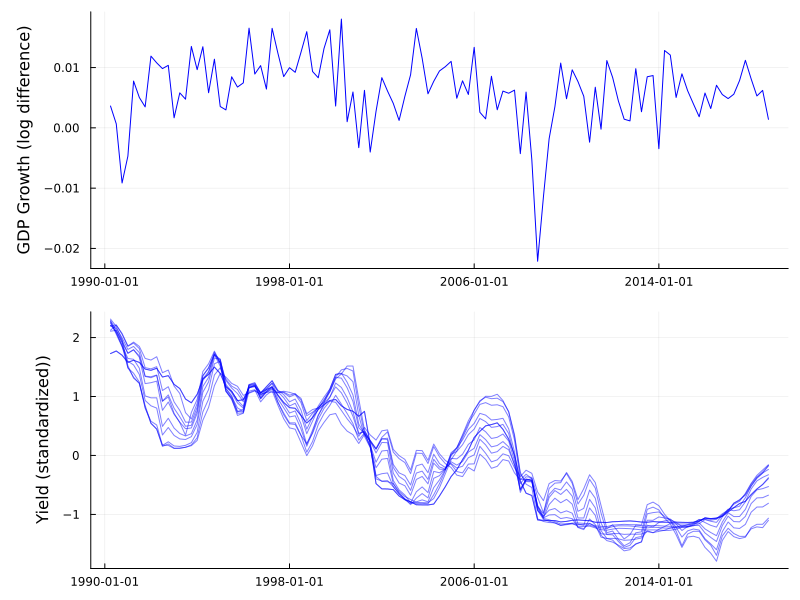
\includegraphics{index_files/mediabag/index_files/figure-pdf/fig-dl-data-output-1.pdf}

}

\caption{\label{fig-dl-data}GDP growth and yield curve data.}

\end{figure}%

\paragraph{Model}\label{model}

Let \(G_t\) denote growth and \(\mathbf{Y}_t\) denote the yield curve at
time \(t\). Then we are interested in a model for \(G_t\) conditional on
\(\mathbf{Y}_t\). Let \(\theta\) denote our model parameters then
formally we are interested in maximizing the likelihood
\(p_{\theta}(G_t|\mathbf{Y}_t)\). To do this, we will use a simple
autoencoder architecture that is illustrated in
Figure~\ref{fig-dl-model}. The encoder will consist of a single fully
connected hidden layer with 32 neurons and a hyperbolic tangent
activation function. The bottleneck layer connecting the encoder to the
decoder is a fully connected layer with 6 neurons. This is the
compressed latent representation of the yield curve mentioned above. The
decoder will consist of two fully connected layers each with a
hyperbolic tangent activation function: the first layer will consist of
32 neurons and the second layer will have the same dimension as the
input data. The output layer will consist of a single neuron with a
linear activation function. The model will be trained using the mean
squared error loss function and the Adam optimizer.

\begin{figure}

\centering{

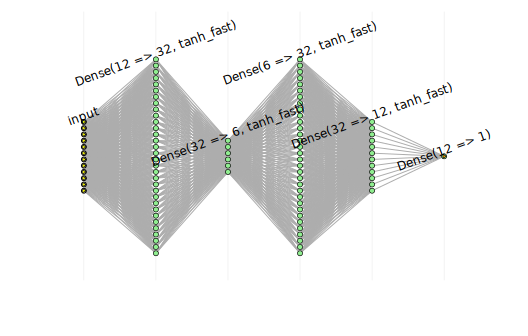
\includegraphics{index_files/mediabag/index_files/figure-pdf/fig-dl-model-output-1.pdf}

}

\caption{\label{fig-dl-model}Model architecture.}

\end{figure}%

\paragraph{Linear Probe}\label{linear-probe}

The results are shown in Figure~\ref{fig-dl-results}. The top panel
shows the actual GDP growth and fitted values from the autoencoder
model. We observe that the model captures the relationship between
economic growth and the yield curve reasonably well. As discussed above,
we also know that the relationship between economic growth and the yield
curve is characterized by two main factors: the level and the spread.
Since the model itself is fully characterized by its parameters, we
would expect that these two important factors are reflected somewhere in
the latent parameter space.

The bottleneck layer seems like a good place to start looking. To get
the latent embeddings \(\mathbf{A}_t\) at time \(t\), we simply pass the
yield curve data \(\mathbf{Y}_t\) through the encoder. Next, we follow
Gurnee and Tegmark (2023) and use a linear probe to regress the observed
yield curve factors on the latent embeddings. Let \(F_t\) denote the
vector containing the two factors of interest in time \(t\):
\(f_t^{\text{spread}}\) and \(f_t^{\text{level}}\). Formally, we are
interested in the following regression model:
\(p_{w}(F_t|\mathbf{A}_t)\) where \(w\) denotes the regression
parameters. Following Gurnee and Tegmark (2023), we use Ridge regression
with \(\lambda\) set to \(0.1\). Using the estimated regression
parameters \(\hat{w}\) we can then predict the yield curve factors from
the latent embeddings: \(\hat{F}_t=\hat{w}^{\prime}\mathbf{A}_t\).

The results of this experiment are shown in the bottom panel of
Figure~\ref{fig-dl-results}. Solid lines show the observed yield curve
factors over time, while dashed lines show predicted values. We find
that the latent embeddings predict the two yield curve factors
reasonably well, in particular the spread. To put this in true
hype-lingo:

\begin{quote}
Not just a parrot! Our autoencoder neural network has an implicit
understanding of the yield curve factors and their relationship with
economic growth. It's sentient indeed!
\end{quote}

\begin{figure}

\centering{

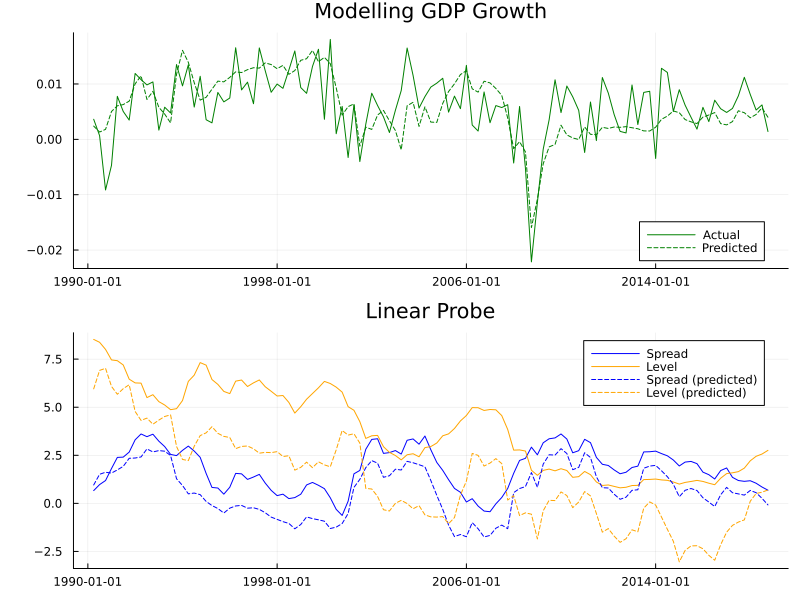
\includegraphics{index_files/mediabag/index_files/figure-pdf/fig-dl-results-output-1.pdf}

}

\caption{\label{fig-dl-results}The top panel shows the actual GDP growth
and fitted values from the autoencoder model. The bottom panel shows the
observed average level and spread of the yield curve (solid) along with
the predicted values from the linear probe based on the latent embedding
(dashed).}

\end{figure}%

\paragraph{Ok, but truly what's the
point?}\label{ok-but-truly-whats-the-point}

The finding is not surprising but it is still interesting. In the
context of mechanistic interpretability, it demonstrates that the
black-box model has evidently learned plausible explanations for the
data. Beyond that, in this particular example, the patterns in the
latent space that we have just uncovered might actually be useful for
downstream tasks. An interesting idea could be to use the latent
embeddings as features in a more traditional and interpretable
econometric model. To demonstrate this, let us consider a simple linear
regression model for GDP growth. We will compare the performance of the
following models: (1) regressing growth \(G_t\) on the latent embedding
\(A_t\), (2) regression growth on the best subset of latent embeddings
\(A_t\), (3) regressing growth on lagged growth, (4) regressing growth
on lagged growth and the observed yield curve factors \(F_t\), (5)
regressing growth on the best subset of yield curve factors \(F_t\),
and, finally, (5) regressing growth on lagged growth and the best subset
of latent embeddings \(A_t\).

The results are shown in the table below. The key finding of interest is
that the coefficients on the latent embeddings in model (5) are
statistically significant. This suggests that the latent embeddings
contain information that is useful for predicting GDP growth.

\begin{tabular}{lrr}
\toprule
              &  \multicolumn{2}{c}{GDP Growth} \\ 
\cmidrule(lr){2-3} 
              &            (1) &            (2) \\ 
\midrule
(Intercept)   &          0.002 &       0.004*** \\ 
              &        (0.002) &        (0.001) \\ 
Lagged Growth &       0.385*** &       0.344*** \\ 
              &        (0.089) &        (0.088) \\ 
Spread        &          0.000 &                \\ 
              &        (0.001) &                \\ 
Level         &          0.000 &                \\ 
              &        (0.000) &                \\ 
Embedding 6   &                &         0.008* \\ 
              &                &        (0.003) \\ 
\midrule
Obs.          &            114 &            114 \\ 
BIC           &       -857.429 &       -864.499 \\ 
R²            &          0.168 &          0.203 \\ 
\bottomrule
\end{tabular}


\subsubsection{Example: Large Language Model}\label{ex-llm}

To round up this section, we will jump back on the hype train and
consider an example involving an LLM. In particular, we will closely
follow the approach in Gurnee and Tegmark (2023) and apply it to a novel
financial dataset: the \emph{Trillion Dollar Words} dataset introduced
by Shah, Paturi, and Chava (2023). The dataset contains a curated
selection of sentences formulated by central bankers of the US Federal
Reserve and communicated to the public in speeches, meeting minutes and
press conferences. The authors of the paper use this dataset to train
LLMs to classify sentences as either `dovish', `hawkish' or `neutral'.
To this end, they first manually annotate a subsample of the available
data and then fine-tune various foundation models. Their model of
choice, \emph{FOMC-RoBERTa} (a fine-tuned version of RoBERTa (Liu et al.
2019)), achieves an \(F_1\) score of around \(>0.7\) for the
classification task. To illustrate the potential usefulness of the
learned classifier, they use predicted labels for the entire dataset to
compute an ad-hoc, count-based measure of `hawkishness'. They then go on
to show that this measure correlates with key economic indicators in the
expected direction: when inflationary pressures rise, the measured level
of `hawkishness' increases as central bankers need to raise interest
rates to bring inflation back to target.

\paragraph{Linear Probes}\label{linear-probes}

Instead of computing a measure based on predicted labels, we can use
linear probes to assess if the fine-tuned model has learned associative
patterns between central bank communications and key economic
indicators. To this end, I have further pre-processed the data provided
by Shah, Paturi, and Chava (2023) and used their proposed model to
compute layer-wise embeddings for all available sentences. I have made
these available and easily accessible through a small Julia package:
\href{https://github.com/pat-alt/TrillionDollarWords.jl}{TrillionDollarWords.jl}.
For each layer, I have then computed linear probes on two inflation
indicators---the Consumer Price Index (CPI) and the Producer Price Index
(PPI)---as well as US Treasury yields at different levels of maturity.
To mitigate issues related to over-parameterization, I follow the
recommendation in Alain and Bengio (2018) to first reduce the
dimensionality of the embeddings each time. In particular, linear probes
are restricted to the first 128 principal components of the embeddings
of each layer.

Detailed results of this experiment will be released in an upcoming
paper. Figure~\ref{fig-fomc} highlights the result for the linear probe
on the CPI. The chart shows various performance measures plotted against
\emph{FOMC-RoBERTa}'s \(n\)-th layer. Shaded areas show the variation
across cross-validation folds, where we have used an expanding window
approach to split the time series. To avoid look-ahead bias, we run PCA
separately for each training set. Results for the linear probes are
shown along with results for autoregressive models (AR) used as our
baseline.

The first column shows the correlations between model predictions and
observed inflation. One can observe that this correlation is strictly
positive for the baseline models and the linear probes. Consistent with
the findings in Gurnee and Tegmark (2023) and Alain and Bengio (2018),
we also observe that this correlation tends to be higher for layers near
the end of the transformer model. Those layers produce predictions that
are more positively correlated with observed inflation than those
produced by the corresponding autoregressive models.

Similarly, we observe that the (root) mean squared error of the linear
probe is largely on par with the baseline. The average prediction error
is gradually reduced as we move along the horizontal axis, which is
again indicative of the notion that layers closer to the end of the
neural network have distilled more useful representations.

\begin{figure}

\centering{

\includegraphics{results/figures/fomc_probe.png}

}

\caption{\label{fig-fomc}Various performance measures (correlation and
(root) mean squared error) plotted against \emph{FOMC-RoBERTa}'s
\(n\)-th layer. Shaded areas indicate variation across cross-validation
folds, where we have used an expanding window approach to split the time
series. Results for the linear probes are shown along with results for
autoregressive models (AR). The optimal lag length was determined using
the Bayes Information Criterium.}

\end{figure}%

\paragraph{Stochastic Parrots After
All?}\label{stochastic-parrots-after-all}

These results from the linear probe shown in Figure~\ref{fig-fomc} are
certainly not unimpressive: even though \emph{FOMC-RoBERTa} was not
explicitly trained to uncover associations between central bank
communications and the level of consumer prices, it appears that the
model has distilled representations that can be used to predict
inflation. It is worth pointing out here that this model is
substantially smaller than the models tested in Gurnee and Tegmark
(2023). This begs the following question:

\begin{quote}
Have we uncovered further evidence that LLMs ``aren't mere stochastic
parrots''? Has \emph{FOMC-RoBERTa} developed an intrinsic understanding
of the economy just by `reading' central bank communications?
\end{quote}

Personally, I am having a very hard time believing this. To argue my
case, I will now produce a counter-example demonstrating that, if
anything, these findings are very much in line with the parrot metaphor.
The counter-example is based on the following premise: if the results
from the linear probe truly were indicative of some intrinsic
understanding of the economy, then the probe should not be sensitive to
random sentences that are most definitely not related to consumer
prices.

To test this, I select the best-performing probe trained on the
final-layer activations to predict changes in the CPI. I then make up
sentences that fall into one of these four categories:
\emph{Inflation/Prices} (IP)---sentences about price inflation,
\emph{Deflation/Prices} (DP)---sentences about price deflation,
\emph{Inflation/Birds} (IB)---sentences about an inflation in the number
of birds and \emph{Deflation/Birds} (DB)---sentences about a deflation
in the number of birds. A sensible sentence for category DP, for
example, could be: ``It is essential to bring inflation back to target
to avoid drifting into deflation territory.''. Analogically, we could
construct the following sentence for the DB category: ``It is essential
to bring the numbers of doves back to target to avoid drifting into
dovelation territory.''.

In light of the encouraging results for the probe in
Figure~\ref{fig-fomc}, we should expect the probe to predict higher
levels of inflation for activations for sentences in the IP category
than for sentences in the DP category. If this was indicative of true
intrinsic understanding, we would not expect to see any significant
difference in predicted inflation levels for sentences about birds,
independent of whether or not their numbers are increasing. More
specifically, we would not expect the probe to predict values for
sentences about birds that are substantially different from the values
it can be expected to predict when using actual white noise as inputs.

To get to this last point, I also generate many probe predictions for
samples of noise. Let \(f: \mathcal{A}^k \mapsto \mathcal{Y}\) denote
the linear probe that maps from the \(k\)-dimensional space spanned by
\(k\) first principal components of the final-layer activations to the
output variable of interest (CPI growth in this case). Then I sample
\(\varepsilon_i \sim \mathcal{N}(\mathbf{0},\mathbf{I}^{(k \times k)})\)
for \(i \in [1,1000]\) and compute the sample average. I repeat this
process \(10000\) times and compute the median-of-means to get an
estimate for \(\mathbb{E}[f(\varepsilon)]=\mathbb{E}[y|\varepsilon]\),
that is the predicted value of the probe conditional on white noise.

Next, I propose the following hypothesis test as a minimum viable
testing framework to assess if the probe results (may) provide evidence
for an actual understanding of key economic relationships learned purely
from text:

\begin{proposition}[Parrot
Test]\protect\hypertarget{prp-line}{}\label{prp-line}

~

\begin{itemize}
\tightlist
\item
  \emph{H0} (Null \emph{WEAK}): The probe never predicts values that are
  statistically significantly different from
  \(\mathbb{E}[f(\varepsilon)]\)
\item
  \emph{H1} (Stochastic Parrots \emph{RISKIER}): The probe predicts
  values that are statistically significantly different from
  \(\mathbb{E}[f(\varepsilon)]\) for sentences in all categories
  (IP,DP,IB,DB).
\item
  \emph{H2} (More than Mere Stochastic Parrots \emph{RISKIEST}): The
  probe predicts values that are statistically significantly different
  from \(\mathbb{E}[f(\varepsilon)]\) for sentences in categories IP and
  DP, but not for sentences in IB and DB.
\end{itemize}

\end{proposition}

To be clear, if in such a test we did find substantial evidence in
favour of rejecting both \emph{HO} and \emph{H1}, this would not
automatically imply that \emph{H2} is true. But to even continue
investigating if based on having learned meaningful representation the
underlying LLM is more than just a parrot, it should be able to pass
this simple test.

In this particular case, Figure~\ref{fig-attack} demonstrates that we
find some evidence to reject \emph{H0} but not \emph{H1} for
\emph{FOMC-RoBERTa}. The median linear probe predictions for sentences
about inflation and deflation are indeed substantially higher and lower,
respectively than for random noise. Unfortunately, the same is true for
sentences about the inflation and deflation in the number of birds,
albeit to a somewhat lower degree.

I should note that the number of sentences in each category is very
small here (10), so the results in Figure~\ref{fig-attack} cannot be
used to establish statistical significance. That being said, even a
handful of convincing counter-examples should be enough for us to
seriously question the claim that results from linear probes provide
evidence against the parrot metaphor. In fact, if there's even a single
sentence for which any

\begin{quote}
Strong alternative hypothesis to address own confirmation bias
Articulating a test to better differentiate
\end{quote}

\begin{figure}

\centering{

\includegraphics{results/figures/attack_inflation.png}

}

\caption{\label{fig-attack}Probe predictions for sentences about
inflation of prices (IP), deflation of prices (DP), inflation of birds
(IB) and deflation of birds (DB). The vertical axis shows predicted
inflation levels subtracted by the average predicted inflation level for
the whole sample period (train and test set).}

\end{figure}%

\subsection*{References}\label{references}
\addcontentsline{toc}{subsection}{References}

\phantomsection\label{refs}
\begin{CSLReferences}{1}{0}
\bibitem[\citeproctext]{ref-alain2018understanding}
Alain, Guillaume, and Yoshua Bengio. 2018. {``Understanding Intermediate
Layers Using Linear Classifier Probes.''}
\url{https://arxiv.org/abs/1610.01644}.

\bibitem[\citeproctext]{ref-gurnee2023language}
Gurnee, Wes, and Max Tegmark. 2023. {``Language Models Represent Space
and Time.''} \url{https://arxiv.org/abs/2310.02207}.

\bibitem[\citeproctext]{ref-liu2019roberta}
Liu, Yinhan, Myle Ott, Naman Goyal, Jingfei Du, Mandar Joshi, Danqi
Chen, Omer Levy, Mike Lewis, Luke Zettlemoyer, and Veselin Stoyanov.
2019. {``RoBERTa: A Robustly Optimized BERT Pretraining Approach.''}
\url{https://arxiv.org/abs/1907.11692}.

\bibitem[\citeproctext]{ref-shah2023trillion}
Shah, Agam, Suvan Paturi, and Sudheer Chava. 2023. {``Trillion Dollar
Words: A New Financial Dataset, Task \& Market Analysis.''}
\url{https://arxiv.org/abs/2305.07972}.

\end{CSLReferences}



\end{document}
